\documentclass{article} % For LaTeX2e
\usepackage{nips13submit_e,times}
\usepackage{hyperref}
\usepackage{url}
\usepackage{tgtermes}
\usepackage{graphicx} % Required for including pictures
\usepackage{wrapfig} % Allows in-line images
\usepackage{amsmath}
\usepackage{amssymb}
\usepackage{booktabs}
\usepackage{amsthm}
\usepackage{algorithm}
\usepackage{caption}
\usepackage{cmap}
%\documentstyle[nips13submit_09,times,art10]{article} % For LaTeX 2.09


\title{Machine Comprehension using Improved Bi-Directional Attention Flow Network}


\author{
Sijun He \\
Stanford University \\
\texttt{sijunhe@stanford.edu} \\
\And
Jiajun Sun \\
Stanford University \\
\texttt{jiajuns@stanford.edu} \\
\And
Mingxiang Chen \\
Stanford University \\
\texttt{ming1993@stanford.edu} \\
}

% The \author macro works with any number of authors. There are two commands
% used to separate the names and addresses of multiple authors: \And and \AND.
%
% Using \And between authors leaves it to \LaTeX{} to determine where to break
% the lines. Using \AND forces a linebreak at that point. So, if \LaTeX{}
% puts 3 of 4 authors names on the first line, and the last on the second
% line, try using \AND instead of \And before the third author name.

\newcommand{\fix}{\marginpar{FIX}}
\newcommand{\new}{\marginpar{NEW}}

\nipsfinalcopy % Uncomment for camera-ready version

\begin{document}


\maketitle

\begin{abstract}

\end{abstract}

\section{Introduction}
\label{introduction}

Machine Comprehension (MC) and Question Answering (QA) were increasingly popular in the past few years. Almost all human knowledge are recorded as text. Just like what we did in school doing reading comprehension questions, extracting information from a specific piece of context would enable artificial intelligence to get to a higher level. Different kinds of natural language processing structures such as Gated Recurrent Unit (GRU) and Long Short Term Memory (LSTM) has been introduced.

These years, there are several QA database that has been released. In this paper, we describe a way using an improved version of bi-directional attention flow for the task of question answering using recently published Stanford Question Answering Dataset (SQuAD) which consisted of approximately 100K question-answer pairs with the context.

The objective of the study was to extract the answer for a given question from a certain context. The model was built based on the previous hierarchical multi-stage bi-directional attention flow (BiDAF)) model (Minjoon Seo et al. 2017) while evaluating the correctness using corresponding F1 score and exact-match (EM) score.

\section{Models}
\label{models}

Our machine learning model (Figure 1) is hierachical multi-stage with 5 layers.

\subsection{Word Embedding Layer}

The word embedding layer maps each individual word into a high-dimension vector space. It is a set of pretrained GloVe word vectors using datasets provided by Wikipedia 2014 and Gigaword 5. The dimensionality of the vectors are 100.

\subsection{Contextual Embedding Layer}

In this layer, we introduced a Bi-directional Long Short-Term Memory (BiLSTM) network as our encoding layer. Contexts and questions will be fed into the network seperately, while the output from each state will all be recorded. Note that the output of which will be 2d-dimension vectors (where d is 100 in our model) due to the concatenation of two output for each direction of the network.

\begin{figure}[h]
\begin{center}
%\framebox[4.0in]{$\;$}
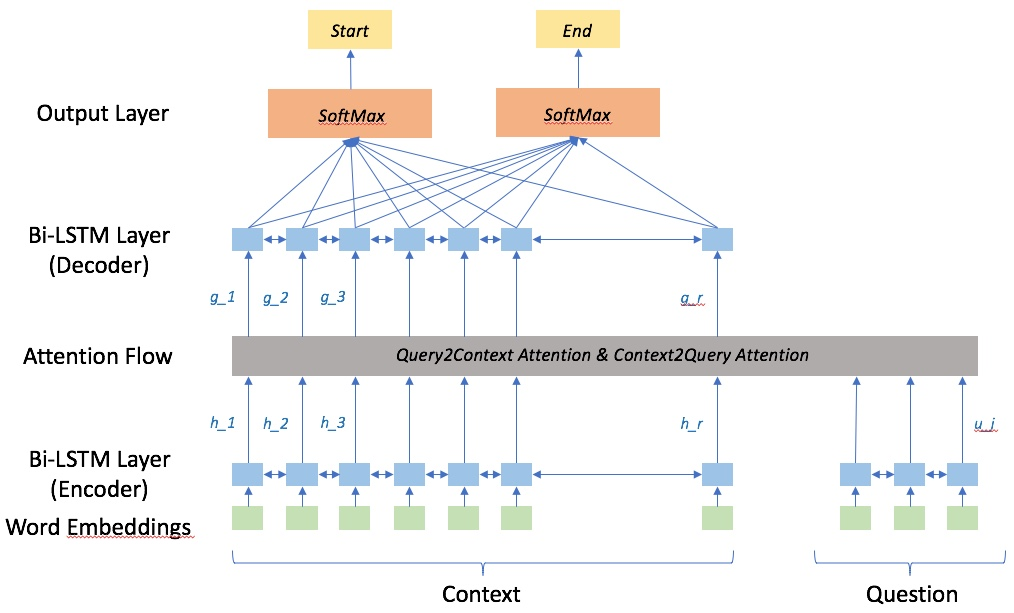
\includegraphics[width=0.9\textwidth]{model_graph.jpeg}
\end{center}
\caption{Bi-Directional Attention Flow Model }
\end{figure}

\subsection{Attention Flow Layer}

The attention layer is introduced to link together the information from the question and the information given by the context. It tells us how important it is that we should pay attention to each word vector in the text (both contexts and questions). The input of this layer is contextual vector of the context H and the question U.

In this layer, the attention is calculated from the similarity matrix of H and U as follow:\\
\newline
\centerline{$S_{ij}=\alpha (H_{:,t}, U(:,j))$}\\
\newline
where $S_ij$ indicates the similarity of the word i in the context and the word j in the query, and $\alpha$ is the bilinear factor which is defined as\\
\newline
\centerline{$\alpha (h,u)=h^TW_{bi}u$}\\
\newline
W is a trainable matrix of $R^{2d\times 2d}$ (Chen et al. 2016).

\subsubsection{Context-to-query Attention}

The context-to-query attention indicates the weight of each word in the query considering the given context. The attention weight is computed as follow\\
\newline
\centerline{$weight=SoftMax(S_{i:})$}\\
\newline
so that the query vectors turn out to be\\
\newline
\centerline{$\hat{U}=\sum_j a_{ij}U_{:j}$}\\

\subsubsection{Query-to-context Attention}

The query-to-context attention indicates the weight of each context word considering the given query. Similar to what we did in context-to-query attention, the attention weights are calculated from\\
\newline
\centerline{$b=SoftMax(max_{col}(S)$}\\
\newline
and
\newline
\centerline{$\hat{H}=\sum_tb_tH_{:t}$}\\
\newline
Then we combined three vectors as the yield G, where $\beta$ is a trainable vector of $R^{8d\times T}$\\
\newline
\centerline{$G=\beta (H, \hat{U}, \hat{H}$}\\

\subsection{Modeling Layer}

The input of the modeling layer (decoding layer) encrypts the information of the context together with some information from the query. So that when we pass the tensor to a bi-LSTM network, similar to what we did in the contextual embedding layer, the output would be a matrix of $R^{2d\times T}$, where T indicates the number of context in the dataset.

\subsection{Output Layer}

In this layer, we provides the answer to questions by calculating the probability for each position in the context as the start and the end of the answer with SoftMax. However, in some situations, though very rare, we would flip over the start and ending labels if the ending predicted maybe even appears earlier than the start in the context. It would be discussed more in detail in section 4.

\section{Headings: first level}
\label{headings}

First level headings are lower case (except for first word and proper nouns),
flush left, bold and in point size 12. One line space before the first level
heading and 1/2~line space after the first level heading.

\subsection{Headings: second level}

Second level headings are lower case (except for first word and proper nouns),
flush left, bold and in point size 10. One line space before the second level
heading and 1/2~line space after the second level heading.

\subsubsection{Headings: third level}

Third level headings are lower case (except for first word and proper nouns),
flush left, bold and in point size 10. One line space before the third level
heading and 1/2~line space after the third level heading.

\section{Citations, figures, tables, references}
\label{others}

These instructions apply to everyone, regardless of the formatter being used.

\subsection{Citations within the text}

Citations within the text should be numbered consecutively. The corresponding
number is to appear enclosed in square brackets, such as [1] or [2]-[5]. The
corresponding references are to be listed in the same order at the end of the
paper, in the \textbf{References} section. (Note: the standard
\textsc{Bib\TeX} style \texttt{unsrt} produces this.) As to the format of the
references themselves, any style is acceptable as long as it is used
consistently.

As submission is double blind, refer to your own published work in the 
third person. That is, use ``In the previous work of Jones et al.\ [4]'',
not ``In our previous work [4]''. If you cite your other papers that
are not widely available (e.g.\ a journal paper under review), use
anonymous author names in the citation, e.g.\ an author of the
form ``A.\ Anonymous''. 


\subsection{Footnotes}

Indicate footnotes with a number\footnote{Sample of the first footnote} in the
text. Place the footnotes at the bottom of the page on which they appear.
Precede the footnote with a horizontal rule of 2~inches
(12~picas).\footnote{Sample of the second footnote}

\subsection{Figures}

All artwork must be neat, clean, and legible. Lines should be dark
enough for purposes of reproduction; art work should not be
hand-drawn. The figure number and caption always appear after the
figure. Place one line space before the figure caption, and one line
space after the figure. The figure caption is lower case (except for
first word and proper nouns); figures are numbered consecutively.

Make sure the figure caption does not get separated from the figure.
Leave sufficient space to avoid splitting the figure and figure caption.

You may use color figures. 
However, it is best for the
figure captions and the paper body to make sense if the paper is printed
either in black/white or in color.
\begin{figure}[h]
\begin{center}
%\framebox[4.0in]{$\;$}
\fbox{\rule[-.5cm]{0cm}{4cm} \rule[-.5cm]{4cm}{0cm}}
\end{center}
\caption{Sample figure caption.}
\end{figure}

\subsection{Tables}

All tables must be centered, neat, clean and legible. Do not use hand-drawn
tables. The table number and title always appear before the table. See
Table~\ref{sample-table}.

Place one line space before the table title, one line space after the table
title, and one line space after the table. The table title must be lower case
(except for first word and proper nouns); tables are numbered consecutively.

\begin{table}[t]
\caption{Sample table title}
\label{sample-table}
\begin{center}
\begin{tabular}{ll}
\multicolumn{1}{c}{\bf PART}  &\multicolumn{1}{c}{\bf DESCRIPTION}
\\ \hline \\
Dendrite         &Input terminal \\
Axon             &Output terminal \\
Soma             &Cell body (contains cell nucleus) \\
\end{tabular}
\end{center}
\end{table}

\section{Final instructions}
Do not change any aspects of the formatting parameters in the style files.
In particular, do not modify the width or length of the rectangle the text
should fit into, and do not change font sizes (except perhaps in the
\textbf{References} section; see below). Please note that pages should be
numbered.

\subsubsection*{Acknowledgments}

Use unnumbered third level headings for the acknowledgments. All
acknowledgments go at the end of the paper. Do not include 
acknowledgments in the anonymized submission, only in the 
final paper. 

\subsubsection*{References}

References follow the acknowledgments. Use unnumbered third level heading for
the references. Any choice of citation style is acceptable as long as you are
consistent. It is permissible to reduce the font size to `small' (9-point) 
when listing the references. {\bf Remember that this year you can use
a ninth page as long as it contains \emph{only} cited references.}

\small{
[1] Danqi Chen., Jason Bolton. \& Christopher D. Manning. (2016) A thorough examination of the cnn/daily mail reading comprehension task. {\it arXiv:1606.02858}



% Reference template. Delete when finished
[1] Alexander, J.A. \& Mozer, M.C. (1995) Template-based algorithms
for connectionist rule extraction. In G. Tesauro, D. S. Touretzky
and T.K. Leen (eds.), {\it Advances in Neural Information Processing
Systems 7}, pp. 609-616. Cambridge, MA: MIT Press.

[2] Bower, J.M. \& Beeman, D. (1995) {\it The Book of GENESIS: Exploring
Realistic Neural Models with the GEneral NEural SImulation System.}
New York: TELOS/Springer-Verlag.

[3] Hasselmo, M.E., Schnell, E. \& Barkai, E. (1995) Dynamics of learning
and recall at excitatory recurrent synapses and cholinergic modulation
in rat hippocampal region CA3. {\it Journal of Neuroscience}
{\bf 15}(7):5249-5262.
}

\end{document}